\documentclass[conference]{IEEEtran}
\IEEEoverridecommandlockouts
% The preceding line is only needed to identify funding in the first footnote. If that is unneeded, please comment it out.
\usepackage{cite}
\usepackage{amsmath,amssymb,amsfonts}
\usepackage{algorithmic}
\usepackage{graphicx}
\usepackage{textcomp}
\usepackage{xcolor}
\def\BibTeX{{\rm B\kern-.05em{\sc i\kern-.025em b}\kern-.08em
    T\kern-.1667em\lower.7ex\hbox{E}\kern-.125emX}}
\begin{document}

\title{Pengembangan \textit{Firmware Tracker} Bus Kampus dengan Modul GNSS pada Platform STM32}

\author{\IEEEauthorblockN{Airlangga Rasyad Fidiyanto, I Wayan Mustika, Agus Bejo}
\IEEEauthorblockA{
Departemen Teknik Elektro dan Teknologi Informasi\\
Universitas Gadjah Mada, Indonesia \\
fairlanggarasyad@mail.ugm.ac.id \{wmustika, agusbj\}@ugm.ac.id}
}

\maketitle

\begin{abstract}
Penelitian ini bertujuan untuk mengevaluasi performa dari modul GNSS Teseo-LIV3FL dan mengembangkan firmware pelacak Bus Trans Gadjah Mada menggunakan platform STM32. Evaluasi performa \textit{multi-constellation} modul dilakukan dengan mengatur modul untuk menerima isyarat dari berbagai konstelasi GNSS. Selain itu, firmware yang dikembangkan memiliki fitur geofencing untuk menentukan apakah posisi bus saat ini berada di dalam lingkungan kampus Universitas Gadjah Mada atau tidak. \textit{Firmware} ini akan diujikan pada Rute 1B Trans Gadjah Mada.
\end{abstract}

\begin{IEEEkeywords}
STM32, Teseo-LIV3FL, pengembangan firmware, pelacakan posisi, algoritma daya rendah, multi-cosntellation
\end{IEEEkeywords}

\section{Pendahuluan}
Bus adalah salah satu moda transportasi dalam kota yang paling populer di Indonesia. Daerah Istimewa Yogyakarta telah menyediakan dua layanan bus publik, yaitu Trans Jogja dan Teman Bus. Salah satu faktor yang membuat penggunaan bus cukup populer adalah cakupan wilayahnya yang luas dan biayanya yang terjangkau \cite{Rohani2013}. Selain itu, lalu lintas yang padat dan lahan parkir yang terbatas juga menjadi motivasi beberapa orang untuk menggunakan transportasi publik. Jika peningkatan jumlah penduduk pada suatu daerah sangat tinggi, maka dibutuhkan fasilitas transportasi umum yang layak seperti bus \cite{Sutandi2015}.

Pada awal bulan Maret 2022, Rektor Universitas Gadjah Mada, Prof. Ir. Panut Mulyono, M.Eng., D.Eng., meluncurkan dua buah bus listrik untuk transportasi internal kampus. Kedua bus ini merupakan inovasi dari UGM untuk memudahkan mobilisasi mahasiswa di area kampus seluas 183,36 hektar dan mengurangi penggunaan energi fosil secara bersamaan. Setiap bus akan memutari UGM sebanyak sepuluh kali dengan setiap putaran membutuhkan satu jam. Dengan adanya fasilitas bus kampus Trans Gadjah Mada diharapkan dapat membuat lingkungan kampus menjadi lebih nyaman dan kondusif.

Salah satu masalah yang banyak dikeluhkan oleh civitas akademika UGM adalah ketidakpastian waktu kedatangan Trans Gadjah Mada. Meskipun sudah diberikan jadwal estimasi kedatangan bus, terkadang waktu kedatangan bus tidak sesuai dikarenakan faktor cuaca, lalu lintas, dan faktor lainnya.

Masalah serupa juga terjadi di India. Berdasarkan penelitian \cite{Sutar2016}, masyarakat India hanya mengetahui waktu kedatangan bus berdasarkan jadwal saja tanpa mengetahui posisi terbaru dari bus yang akan ditumpangi. Penelitian yang dilakukan oleh \cite{Sneha2014} menunjukkan bahwa sistem pelacak berbasis GPS telah diimplementasikan di beberapa negara, tetapi belum diimplementasikan di Indonesia, khususnya di lingkungan Universitas Gadjah Mada.

Untuk mengatasi masalah ketidakpastian waktu kedatangan Trans Gadjah Mada, dibutuhkan sistem pelacakan yang akurat dan terpercaya. Salah satu teknologi sistem navigasi berbasis satelit yang dapat menunjukkan posisi secara akurat adalah Global Navigation Satellite System (GNSS). Dengan dikembangkannya firmware sistem pelacak lokasi bus Trans Gadjah Mada berbasis GNSS, diharapkan dapat membantu untuk melacak posisi bus secara akurat dan meningkatkan kepuasan pengguna.

\section{Penelitian Terkait}
Penelitian sebelumnya telah mengembangkan berbagai sistem pelacak kendaraan dengan berbagai macam pendekatan pada perangkat keras maupun perangkat lunak untuk berbagai aplikasi. Sebagai contoh, \cite{Ekhsan2022} merancang suatu sistem untuk melacak dompet dengan menggunakan TK-102 GPS Tracker.

Tim peneliti dari \textit{Vidyalankar Institute of Technology} telah merancang suatu sistem yang dapat mendeteksi lokasi dari kendaraan dan juga emisi CO yang dihasilkan. Pada sistem yang dirancang, digunakan \textit{development board} Arduino Uno yang berbasis mikrokontroler ATmega328. Ketika kandungan gas CO sudah melebihi ambang batas, sistem akan memutus pengiriman bahan bakar dan kemudian mengirimkan data koordinat dari modul GPS ke \textit{server} Apache yang telah dirancang \cite{Asha2022}.

Sebuah sistem \textit{speedometer} telah dirancang oleh \cite{Najmurrokhman2021}. Sistem tersebut menggunakan modul GPS untuk menghitung kecepatan dan koordinat lokasi kendaraan. Data kecepatan kendaraan didapat dari menghitung waktu yang dibutuhkan oleh kendaraan untuk berpindah dari satu titik ke titik lainnya. Data yang didapat dikirimkan dengan API Adafruit IO menggunakan modul SIM808.

Penelitian yang dilakukan oleh \cite{Mukhtar2015} dari \textit{University of London} menggunakan mikrokontroler AT89S52 dari keluarga 8051. Digunakan modul GPS M-89 yang diatur untuk menerima isyarat transmisi satelit pada frekuensi 1575.42 MHz. Data yang diterima akan ditampilkan pada layar LCD dan dikirimkan dengan modul GSM. Kemudian, data yang telah diterima akan ditampilkan pada situs web.

Sistem yang dirancang pada penelitian \cite{Widya2016} menggunakan modul GPS u-Blox Neo 6m. Penelitian ini memiliki kesamaan, yaitu objek yang akan dilacak adalah kendaraan bus. Sama seperti penelitian-penelitian sebelumnya, pada penelitian ini hanya digunakan satu buah konstelasi GNSS, yaitu GPS.

Namun, pada penelitian-penelitian di atas hanya digunakan satu buah konstelasi GNSS, yaitu GPS. Oleh karena itu, pada penelitian ini akan dirancang sistem pelacak kendaraan berbasis GNSS \textit{multi-constellation} dengan menggunakan modul GNSS Teseo-LIV3FL dan mikrokontroler STM32 WL55JC. Selain itu, sistem \textit{geofencing} yang telah ada dapat dikembangkan lebih lanjut seperti dapat mendeteksi apakah kendaraan sedang berhenti di halte atau tidak. Dengan begitu, penelitian ini diharapkan dapat memberikan kontribusi yang signifikan pada pengembangan sistem pelacak kendaraan berbasis GNSS.

\section{Metode Penelitian}
Penelitian ini dilakukan pada tahun 2023 menggunakan modul GNSS Teseo-LIV3FL dan \textit{development board} STM32 Nucleo-WL55JC1. Lokasi penelitian berada di lingkungan Universitas Gadjah Mada dan sekitarnya. Adapun konfigurasi konstelasi yang digunakan adalah GPS, BeiDou, Galileo, dan QZSS.

\textit{Rapid Static Survey} dilakukan untuk meninjau performa modul GNSS dalam keadaan diam. Pengujian dilakukan dengan meletakan modul di satu tempat dan merekam data selama satu jam. Untuk menerima kalimat NMEA dari modul, digunakan perangkat USB \textit{to} TTL dengan konfigurasi \textit{baud rate} 9600 bps. Pengujian ini dilakukan dalam empat buah skenario, yaitu \textit{basement}, dalam ruangan, ruang semi terbuka, dan ruang terbuka. Lokasi setiap skenario \textit{Rapid Static Survey} ditunjukan oleh Tabel \ref{tab: rss-location}.

\begin{table}[hbt!]
	\caption{Lokasi Pengujian \textit{Rapid Static Survey}}
	\centering
	\renewcommand{\arraystretch}{1.5}
	\begin{tabular}{cc}
		\hline
		\textbf{Skenario} & \textbf{Lokasi} \\\hline
		\textit{Basement} &Ruang Bawah Tanah Fisipol UGM\\
		Dalam Ruangan & Lantai 5 SGLC Fakultas Teknik UGM\\
		Ruangan Semi Terbuka &  Selasar Grha Sabha Pramana\\
		Ruang Terbuka & Lapangan Pancasila\\
		\hline
	\end{tabular}
	\label{tab: rss-location}
\end{table}

Fitur \textit{geofencing} berfungsi untuk memantau posisi dari suatu aset dalam wilayah tertentu. Pada penelitian ini, \textit{geofence} didefinisikan sebagai lingkaran dengan radius satu kilometer dengan pusat di koordinat (-7,771376; 110,377493). Pengujian dilakukan pada delapan belas titik acak di sekitar Universitas Gadjah Mada. \textit{Firmware} akan mengembalikan nilai satu jika posisi saat ini berada di dalam wilayah \textit{geofence} dan nol untuk sebaliknya.

Setelah meninjau performa \textit{multi-constellation} pada modul GNSS dan \textit{geofence}, langkah selanjutnya adalah menguji sisetm secara keseluruhan di Bus Trans Gadjah Mada. Pada penelitian ini, rute yang dipilih adalah Rute 1B (Gambar \ref{fig: tgm-1b}). Waktu tempuh pengujian ini kurang lebih adalah selama satu jam.

\begin{figure}[hbt!]
	\centering
	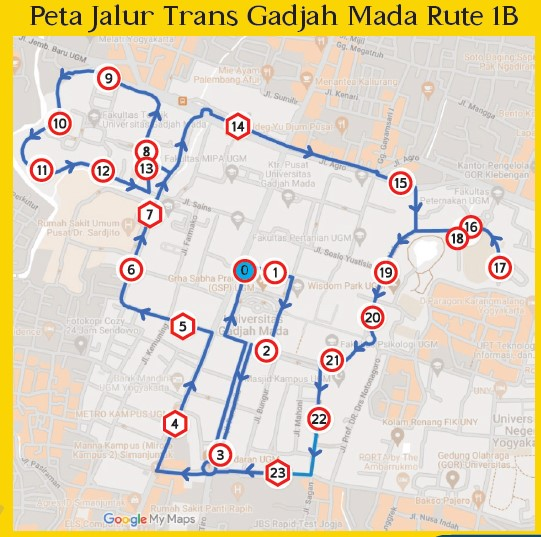
\includegraphics[width=6cm]{Peta-Jalur-Rute-1B.jpg}
	\caption{Rute 1B Trans Gadjah Mada}
	\label{fig: tgm-1b}
\end{figure}

\section{Hasil Pengujian}
\subsection{\textit{Rapid Static Survey}}
\subsection{\textit{Geofencing}}
\subsection{Pengujian pada Bus Trans Gadjah Mada}

\section{Kesimpulan}

%Please number citations consecutively within brackets \cite{b1}. The 
%sentence punctuation follows the bracket \cite{b2}. Refer simply to the reference 
%number, as in \cite{b3}---do not use ``Ref. \cite{b3}'' or ``reference \cite{b3}'' except at 
%the beginning of a sentence: ``Reference \cite{b3} was the first $\ldots$''
%
%Number footnotes separately in superscripts. Place the actual footnote at 
%the bottom of the column in which it was cited. Do not put footnotes in the 
%abstract or reference list. Use letters for table footnotes.
%
%Unless there are six authors or more give all authors' names; do not use 
%``et al.''. Papers that have not been published, even if they have been 
%submitted for publication, should be cited as ``unpublished'' \cite{b4}. Papers 
%that have been accepted for publication should be cited as ``in press'' \cite{b5}. 
%Capitalize only the first word in a paper title, except for proper nouns and 
%element symbols.
%
%For papers published in translation journals, please give the English 
%citation first, followed by the original foreign-language citation \cite{b6}.



\bibliography{references}{}
\bibliographystyle{IEEEtran}

%\begin{thebibliography}{00}
%\bibitem{b1} G. Eason, B. Noble, and I. N. Sneddon, ``On certain integrals of Lipschitz-Hankel type involving products of Bessel functions,'' Phil. Trans. Roy. Soc. London, vol. A247, pp. 529--551, April 1955.
%\bibitem{b2} J. Clerk Maxwell, A Treatise on Electricity and Magnetism, 3rd ed., vol. 2. Oxford: Clarendon, 1892, pp.68--73.
%\bibitem{b3} I. S. Jacobs and C. P. Bean, ``Fine particles, thin films and exchange anisotropy,'' in Magnetism, vol. III, G. T. Rado and H. Suhl, Eds. New York: Academic, 1963, pp. 271--350.
%\bibitem{b4} K. Elissa, ``Title of paper if known,'' unpublished.
%\bibitem{b5} R. Nicole, ``Title of paper with only first word capitalized,'' J. Name Stand. Abbrev., in press.
%\bibitem{b6} Y. Yorozu, M. Hirano, K. Oka, and Y. Tagawa, ``Electron spectroscopy studies on magneto-optical media and plastic substrate interface,'' IEEE Transl. J. Magn. Japan, vol. 2, pp. 740--741, August 1987 [Digests 9th Annual Conf. Magnetics Japan, p. 301, 1982].
%\bibitem{b7} M. Young, The Technical Writer's Handbook. Mill Valley, CA: University Science, 1989.
%\end{thebibliography}



\end{document}
